\section{Continuous-Stream Results}
\label{sec:narrative-results}

\subsection{Timely Attribution and Extra Alarms Measure Different Outcomes}

\begin{table}[t]\centering\small
\caption{H04 with the original publication policies. ExtraTrees rows are archived R09 comparators. Load and line columns require the correct family and source emitted before OFF. The 54 realizations repeat 18 interventions across three R/X conditions; they are not 54 independent trials. Normal exposure is only 204 s per method.}
\label{tab:narrative-results}
\setlength{\tabcolsep}{3pt}\begin{tabular}{lrrrr}\toprule
Method & \shortstack{Load\\timely} & \shortstack{Line\\timely} & Extras & \shortstack{Normal\\alarms}\\\midrule
Physical (5 models) & 26/27 & 27/27 & 4 & 0\\
Physical nominal & 27/27 & 27/27 & 7 & 0\\
Archived ET ref. & 0/27 & 27/27 & 3 & 0\\
Archived ET short & 0/27 & 27/27 & 3 & 0\\
Onset witness & 25/27 & 27/27 & 0 & 0\\
\bottomrule\end{tabular}\end{table}


In H04, both ExtraTrees adapters and both physical references identify all tested lines in time (Table~\ref{tab:narrative-results}). The difference is in loads: the five-model bank obtains \NarMixLoadTimely{}/\NarMixLoadTotal{} timely decisions, nominal \NarNomLoadTimely{}/\NarNomLoadTotal{}, and these ExtraTrees adapters \NarETLoadTimely{}/\NarETLoadTotal{}. This tests transfer of the frozen adapters; it neither rules out supervised load detection nor reproduces the historical multi-class hackathon score.

The five-model bank detects and eventually attributes \NarMixJoint{}/\NarMixEvents{} realizations, but only \ContMixTimely{} diagnoses precede physical OFF. Nominal has \ContNomTimely{} timely diagnoses, with \ContNomExtras{} extras versus \ContMixExtras{}. Detection, eventual attribution and timely attribution therefore give different answers. Representing model uncertainty trades an additional late diagnosis for fewer extra alarms here.

\subsection{Recovery and a New Event Must Remain Competing Explanations}

Figure~\ref{fig:narrative-rolling} shows what the counts omit. The physical state continues evolving after OFF. Retained cause/recovery histories explain that trajectory without resetting the network; a later source must compete against both no-new-event recovery and other interventions.



The out-of-bank BUS31 case shows a remaining timing failure: the source is recovered eventually but too late. The network mixture changes how much mass is assigned to that source, and \eqref{eq:continuous-delta} separates that revision from within-model evidence. This is what the array adds to the explanation. The figure does not establish that a tensor representation alone improves accuracy.

\begin{figure}[!htbp]\centering
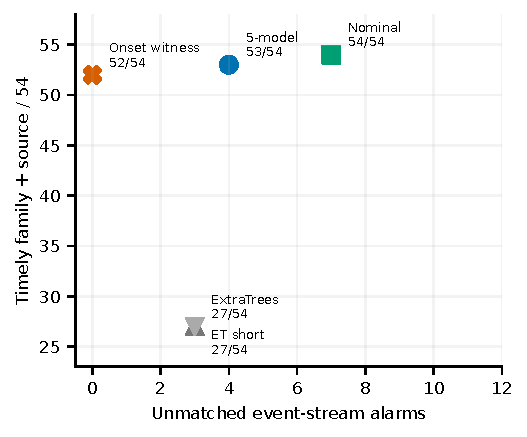
\includegraphics[width=\columnwidth]{figures/generated/narrative_tradeoff.pdf}
\caption{The decision that an accuracy-only table hides. H04 development outcomes trade timely attribution against unmatched event-stream alarms. The onset-witness ablation removes all extras but loses a real BUS16 intervention; it is retained as negative evidence. Labels use 54 paired realizations of 18 interventions and do not imply 54 independent trials.}
\label{fig:narrative-tradeoff}\end{figure}

The onset-witness ablation obtains zero extras but only \ContAdmissionTimely{}/\ContAdmissionTotal{} timely attributions: weak early evidence rejects a real BUS16 load. It inherits the physical states and masses, so suppressing the alarm does not repair the underlying explanation. This negative experiment leaves R11 and nominal frozen for C01.

\begin{figure*}[p]\centering
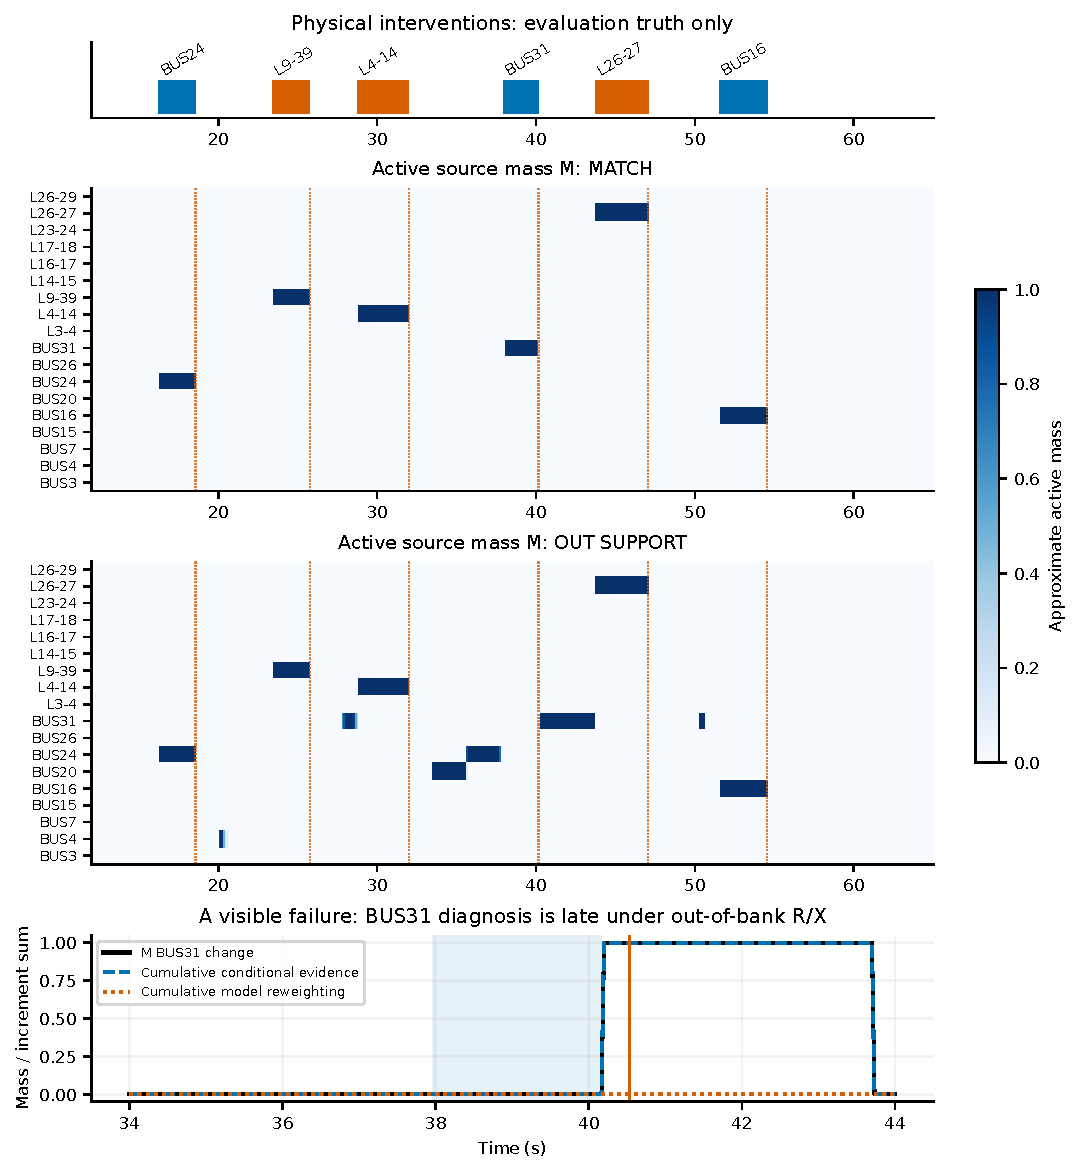
\includegraphics[width=.95\textwidth]{figures/generated/narrative_rolling.pdf}
\caption{From a continuous sequence to source attribution. Top: reserved physical ON--OFF intervals in development parent H002. Middle: active masses for nominal-network observations (MATCH) and mixed R/X changes outside the bank (OUT SUPPORT). Orange dotted lines mark true OFF for evaluation only. Bottom: BUS31 in the latter record; the cumulative terms of $\Delta M$, rebased at 34 s, sum to the change in active mass. Diagnosis arrives after OFF. The figure shows an eventual correct source that fails timely attribution; the color scale represents approximate mass, not calibrated probability.}
\label{fig:narrative-rolling}\end{figure*}
